\documentclass{../qh_assignment}
\graphicspath{ {./images/} }

\begin{document}

\section{Pong}
Voor deze opdracht zul je het klassieke spel Pong gaan maken. Als je nog nooit gehoord hebt van dit spel moet je het even opzoeken om te weten waar we het over hebben (zoek op \texttt{pong game}). Je sketch moet minimaal aan de volgende eisen voldoen. Je bent verder helemaal vrij extra functionaliteit toe te voegen. 
\begin{itemize}
    \item Een bal
    \item Een door de gebruiker bestuurbaar batje
    \item Stuiter-functionaliteit
\end{itemize}
Om je een beetje te helpen staat er onderaan een stappenplan. Je hoeft dit niet te volgen, maar is wel aan te raden als je het moeilijk vind.
    
\begin{enumerate}
    \item Gebruik het volgende opzetje:
    \begin{lstlisting}
      ArrayList<Wall> walls = new ArrayList();
      Wall paddle;
      Ball ball;
      
      void setup() {
        size(500, 500);
        Wall top = new Wall(0,0,width,20);
        Wall right = new Wall(width - 20,0,width - 20,height);
        Wall bottom = new Wall(0,height - 20,width,height - 20);
        paddle = new Wall(0,height / 3,20,height / 4);
        
        walls.add(top);
        walls.add(right);
        walls.add(bottom);
        walls.add(paddle);
       
        ball = new Ball();
      }
      
      void draw() {
        background(255);
        for (Wall w : walls) {
          w.draw();
          ball.bounceIfHits(w);
        }
        ball.draw();
        ball.move();
      }
    \end{lstlisting}
    
    \item Maak de \textbf{Wall} class:
    \begin{lstlisting}
    class Wall {
       int x;
       int y;
       int w;
       int h;
       
        Wall(int x, int y, int w, int h) {
          //TODO
        }
        
        void draw() {
          //TODO
        }
    }  
    \end{lstlisting}
    \tip{Test je code nu al, anders moet je straks een heleboel bugs oplossen!}
    \item Maak de \textbf{Ball} class.
    \begin{lstlisting}
    class Ball {
        PVector pos;
        PVector vel; 
        int radius = 20;
        
        Ball () {
            //TODO
        }
        
        void move() {
            //TODO
        }
        
        void bounceIfHits(Wall w) {
            //TODO
        }
        
        void draw() {
          //TODO
        }
    }
    \end{lstlisting}
    \item Maak als laatste de besturing van \textbf{paddle}!
\end{enumerate}
\begin{figure}[H]
	\centering
	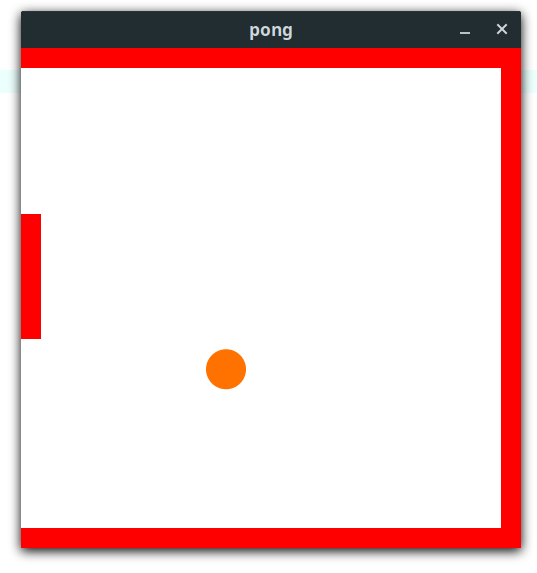
\includegraphics[width=0.5\textwidth]{pong.png}
	\caption{Een voorbeeld van Pong}
	\label{fig:koch}
\end{figure}

\newpage

\section{Bonus functionaliteit}
Voeg extra features aan je sketch toe. Hier onder is een lijst met voorbeelden van extra dingen, je mag natuurlijk ook zelf iets leuks bedenken.
\begin{itemize}
    \item Restarten
    \item Geef het badje een andere kleur (gebruik inheritance).
    \item Het bijhouden van de score (en tonen op het scherm)
    \item Meerdere ballen tegelijk
    \item Multiplayer (geef de andere speler twee andere toetsen)
    \item Power-ups
    \item Meerdere levels
\end{itemize}

\end{document}